\chapter{Objetivos}

\label{Chapter2} % Change X to a consecutive number; for referencing this chapter elsewhere, use \ref{ChapterX}

Una vez presentado el contexto, en este capítulo se abordarán los objetivos que se pretenden alcanzar. Tras una descripción del problema y unos requisitos obligatorios, se detallará la metodología y la planificación que se ha llevado a cabo en la elaboración de este trabajo.

%------------------------------------------------
%	SECTION Descripción del problema
%------------------------------------------------
\section{Descripción del problema}

El objetivo principal de este trabajo es desarrollar una solución al problema SLAM.

A través de técnicas de odometría visual incrementales, se ha construido un sistema capaz de averiguar la posición y orientación de un sensor RGBD que se mueve libremente por el espacio y que va alimentando al sistema con las imágenes obtenidas en tiempo real.

A fin de abordar el objetivo principal de la manera más simple se han propuesto los siguientes subobjetivos:

\begin{enumerate}
\item \underline{Actualización de los datos del sensor}.
Creación de un módulo encargado de recoger de manera dinámica las imágenes RGB y DEPTH del sensor, y actualizarlas en una memoria compartida.
 
\item \underline{Detección de puntos de interés}.
Creación de un componente capaz de recoger a través de diferentes técnicas puntos de interés de una imágen con la opción de desarrollar algún filtro para añadir robustez a la detección.

\item \underline{Emparejamiento de puntos}.
Desarrollo de una funcionalidad encargada de relacionar los puntos de interés previamente obtenidos, a través de técnicas como Fuerza bruta o FLANN.

\item \underline{Estimación del movimiento}.
Implementación de la matemática necesaria para una vez tenidos los puntos emparejados calcular la matriz de rotación y traslación (RT) que se necesitará para calcular en ese instante el movimiento de la cámara.

\item \underline{Pruebas y experimentos}.
Ejecución de la aplicación con objetivo de ajustar, pulir y validar las funciones y algoritmos realizados.

\end{enumerate}

%------------------------------------------------
%	SECTION Requisitos
%------------------------------------------------
\section{Requisitos}

A parte de los requisitos mencionados en el apartado anterior. La implementación y solución final del proyecto debe satisfacer además los siguientes puntos:

\begin{itemize}

\item Desarrollo del proyecto haciendo uso de la plataforma \textbf{JDeRobot 5.4.0}, que ha resultado de mucha utilidad y ha permitido un ahorro significante de tiempo, ya que permite abstraerse de algunas de las funcionalidades de más bajo nivel como puede ser la captura de información del sensor o el protocolo de comunicaciones. Permite llevar un desarrollo modular y el aprovechamiento de componentes ya implementados en la plataforma. Tanto las ventajas como el uso de JDeRobot se tratarán en detalle en el siguiente capítulo  (\ref{Chapter3}).

\item Como la mayoría de componentes están en C++, el trabajo también se ha desarrollado utilizando el mismo lenguaje de programación. 
%~\ref{ch:Chapter3}.

\item Funcional bajo sistema operativo linux, en este caso Ubuntu 14.04 LTS.

\item Uso exclusivo de un único sensor RGBD.

\item Implementación de una interfaz de usuario clara donde se pueda apreciar el proceso de estimación de posición. Incluyendo un entorno visual 3D donde se refleje la posición y movimiento de la cámara en tiempo real.

\end{itemize}


%------------------------------------------------
%	SECTION Metodología
%------------------------------------------------
\section{Metodología}

Para abordar un proyecto de tal envergadura es necesaria una metodología de desarrollo para ir progresando de una manera ordenada y efectiva. En este caso se ha optado por el modelo en espiral basado en prototipos propuesto por B. Boehm en 1986 \parencite{Reference7}, ya que permite el desarrollo de una manera progresiva e incremental. 

Esta metodología permite el desarrollo de implementaciones parciales que van siendo probadas a medida que después de cada ciclo se va generando un prototipo más completo de lo que incorpora el ciclo anterior. Por lo tanto, en cada ciclo o iteración se va añadiendo complejidad a la vez que se van generando funcionalidades nuevas.

Este modelo, utilizado en el trabajo, ha servido de gran ayuda, ya que permite ir avanzando de menos a más, con unos requisitos dependientes de los anteriores y a la vez diferentes para cada iteración. Además permite ir evaluando y adaptando la evolución del desarrollo a nuestros intereses, algo que suele ocurrir normalmente en los proyectos de investigación.

En la Figura~\ref{fig:spiral} se puede observar el ciclo completo de desarrollo de software en el modelo en espiral. Cada etapa o ciclo completo está compuesto por cuatro fases:

\begin{itemize}
\item \underline{Identificación de objetivos}. En esta primera fase se deciden y se planifican los objetivos a alcanzar en la siguiente iteración partiendo de lo realizado en el ciclo anterior. En caso de la primera iteración se definen los objetivos iniciales.

\item \underline{Evaluación alternativa}. Aquí se definen requisitos y se estudian las distintas maneras de abordar los objetivos marcados de la etapa anterior. Se estudian los riesgos y se evaluan de manera que se puedan reducir lo máximo posible. Se debe tener un prototipo antes de la siguiente etapa.

\item \underline{Desarrollo del producto}. En esta fase se diseña y se implementa el producto en base a lo planteado en las anteriores fases. Por último, se verifica y se prueba.

\item \underline{Planificación de la siguiente fase}. Considerando el resultado de la fase anterior, se planifica la siguiente considerando los errores cometidos y los resultados esperados, comenzando así una nueva iteración.

\end{itemize}

\begin{figure}[th]
\centering
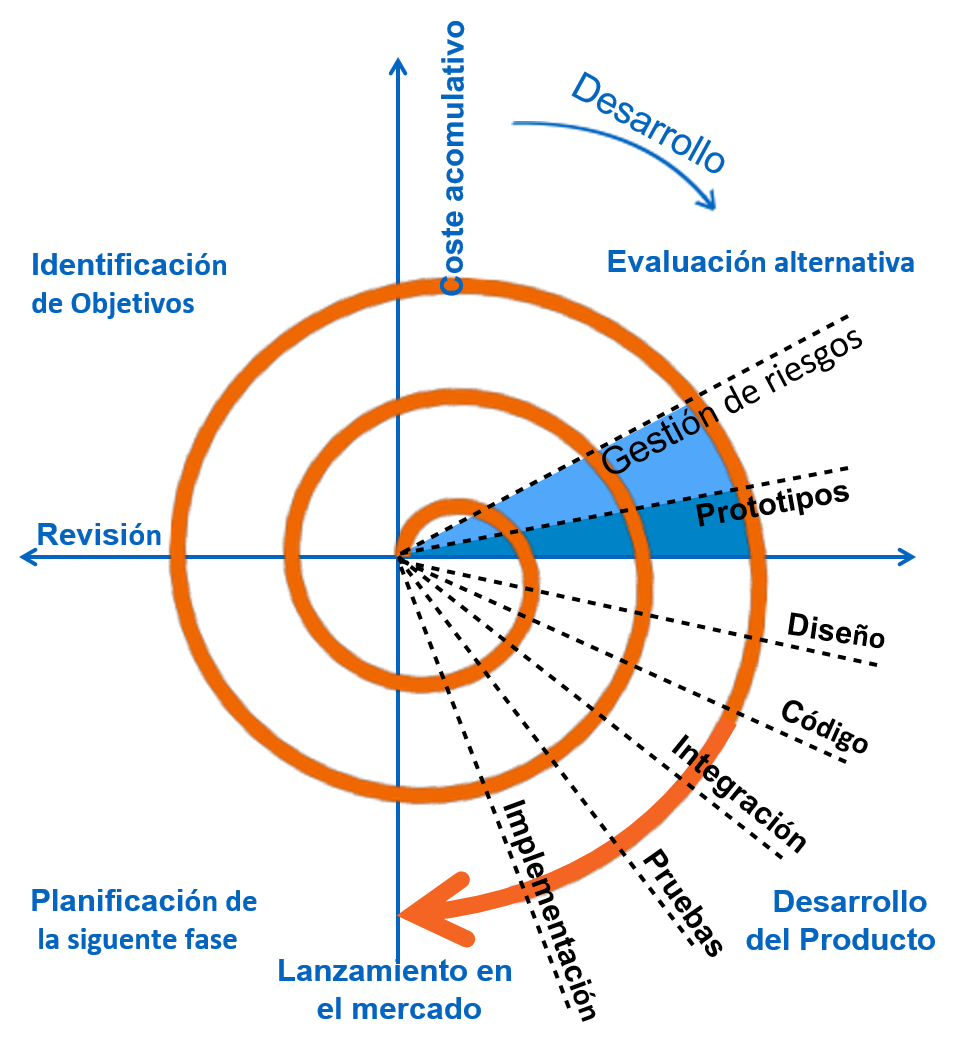
\includegraphics[scale=0.62]{Figures/spiral.png}
\decoRule
\caption[Ciclo de vida en espiral]{Ciclo de vida del desarrollo del \textit{software} en el modelo espiral.}
\label{fig:spiral}
\end{figure}

En la siguiente sección se detallarán los ciclos que han seguido a lo largo de este proyecto. Para las fases de planificación y análisis se han mantenido reuniones semanales con el tutor, con intención de revisar, resolver problemas y encarar los nuevos objetivos establecidos.

A fin de documentar y guardar los hitos realizados en el desarrollo del proyecto, así como los errores cometidos y su posible solución, se ha llevado un seguimiento en mediawiki\footnote{http://jderobot.org/J.benitod-tfg} con los detalles de las diferentes iteraciones, ayudadas a veces por imágenes y/o vídeos.

Para la gestión de código se han usado herramientas \textit{software} de control de versiones, primeramente con Subversion (SVN)\footnote{http://svn.jderobot.org/users/j.benitod/pfc} y finalmente con GIT en un repositorio de GitHub\footnote{https://github.com/RoboticsURJC-students/2014-pfc-Javier-Benito}.

%------------------------------------------------
%	SECTION Planificación
%------------------------------------------------
\section{Planificación}

A lo largo del trabajo se han ido proponiendo etapas asesoradas y con supervisión del tutor. Las más importantes caben destacar:

\begin{enumerate}

\item \textbf{Familiarización de la herramienta JDeRobot}.

Esta etapa consistió en la instalación y el estudio de la plataforma, profundizando en el uso de algún componente con un objetivo muy concreto y sencillo.

Después, y para entender el funcionamiento de algunos de los componentes a bajo nivel más importantes para el trabajo, se propuso el desarrollo de algunos de ellos en otros lenguajes de programación tales como Java o Python.

\item \textbf{Aprendizaje de las herramientas específicas}.

Aquí, a través de prácticas muy concretas se entendió el funcionamiento de algunas de las librerías esenciales para la práctica final.

\begin{itemize}

\item Se realizó un componente utilizando \textbf{PCL} para el cálculo de planos desde nubes de puntos.

\item Se utilizó \textbf{Eigen} para otra práctica en el cálculo de sistemas sobredimensionados de ecuaciones, con descomposición QR y en valores singulares (SVD) resolviendo en diferentes casos una recta de regresión para distintos escenarios.

\item \textbf{GSL}, para el cálculo de un componente rectificador de imágenes (Figura~\ref{fig:spiral}).

\begin{figure}[th]
\centering
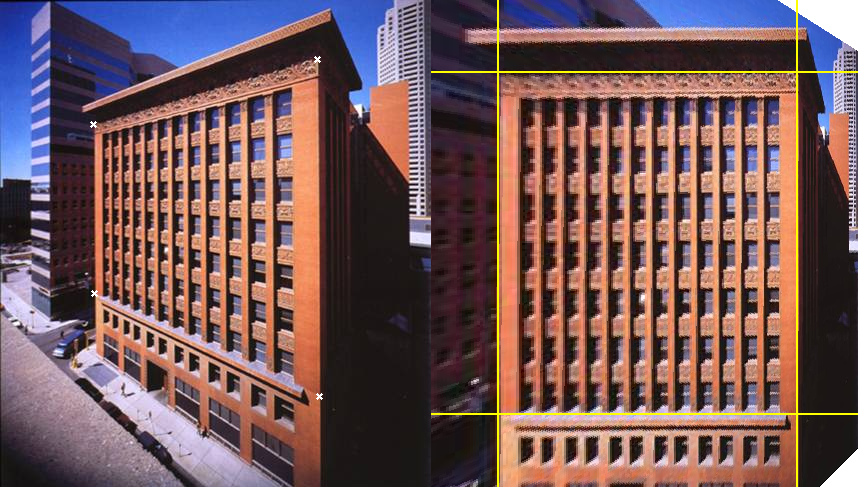
\includegraphics[scale=0.5]{Figures/rectifier.png}
\decoRule
\caption[Componenete rectificador]{Componente rectificador de imágenes.}
\label{fig:rectifier}
\end{figure}


\end{itemize}

\item \textbf{Implementación de un algoritmo para el cálculo de la matriz RT}.

En esta parte se propuso una práctica que sirvió de base para la parte final en la que desde una nube de puntos y otra multiplicada por una matriz RT inventada, se sacaría a través de SVD dicha matriz a partir de las nubes de puntos iniciales y con la opción también de añadir ruido gaussiano a una de ellas. En la Figura~\ref{fig:rtsvd} se encuentra el esquema realizado.

\begin{figure}[th]
\centering
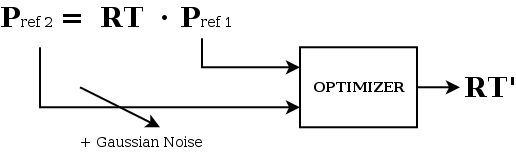
\includegraphics[scale=0.6]{Figures/rt_svd.png}
\decoRule
\caption[Esquema de cálculo de matriz RT]{Esquema de la práctica de cálculo de matriz RT.}
\label{fig:rtsvd}
\end{figure}

\item \textbf{Creación de un componente para la extración de puntos de interés y emparejamiento}.

Aquí se empezó a desarrollar la práctica final, en donde se comenzó por la extracción de puntos de interés con SIFT de las imágenes y los diferentes algoritmos para los emparejamientos. Como esta parte corresponde al desarrollo de la práctica final será detallada en el capítulo \ref{Chapter4}.

\item \textbf{Integración y pruebas experimentales}.

Esta fue la etapa más larga y costosa, ya que el objetivo era dar una solución funcional al problema propuesto. Surgieron multitud de errores que se tuvieron que ir depurando con cada iteración, proponiendo soluciones y alternativas. Fueron necesarias numerosas pruebas para conseguir un desarrollo capaz de aportar una solución estable. Esta etapa también será detallada en los siguientes capítulos, en concreto en los capítulos \ref{Chapter4} y \ref{Chapter5}.

\end{enumerate}